\chapter{Convolutional Neural Networks}\label{sec-cnn}

\section{Deep Learning}

Deep learning~\cite{lecun2015deep, Goodfellow-et-al-2016-Book} is part of a broader family of machine learning methods that focus on representation learning. Unlike rule based methods used in early days of artificial intelligence, deep learning targets at tasks that are easy for people to perform but hard for people to describe formally---problems that we solve intuitively. Former methods have proved success in problems that can be completely described by a very brief list of completely formal rules, thus easily provided ahead of time by the programmer. That led to the defeat of world chess champion Garry Kasparov by IBM's Deep Blue chess-playing system in 1997~\cite{hsu2002behind}. However, rule based or knowledge based methods fail at intuitive tasks such as recognizing objects or speech. The reason behind this inability is because these tasks require immense amount of knowledge about the world, and much of this knowledge is subjective and intuitive, thus difficult to articulate in a formal way. The difficulties faced by AI systems relying on hard-coded knowledge suggest that AI systems need the ability to acquire their own knowledge, by extracting patterns from raw data, just like how human learns from experiences. This capability is known as machine learning. It does not take long for people to realize that performance of machine learning algorithms depends heavily on the representation of data fed into these algorithms. Under a good representation, factors of variation can be disentangled and non important factors will be discarded. People used to put lots of efforts on hand designing features to get a good representation for every domain specific problem. Unfortunately seeking a good representation for a problem can be as difficult as solving the problem itself. Deep learning solves this central problem in representation learning by introducing representations that are expressed in terms of other, simpler representations. Deep learning allows the computer to build complex concepts out of simpler concepts, thus achieves great power and flexibility by representing the world as a nested hierarchy of concepts. Fig~\ref{fig:ch3-dlrelation} shows a hierarchy relation from AI to deep learning.

\begin{figure}[t]
    \centering
    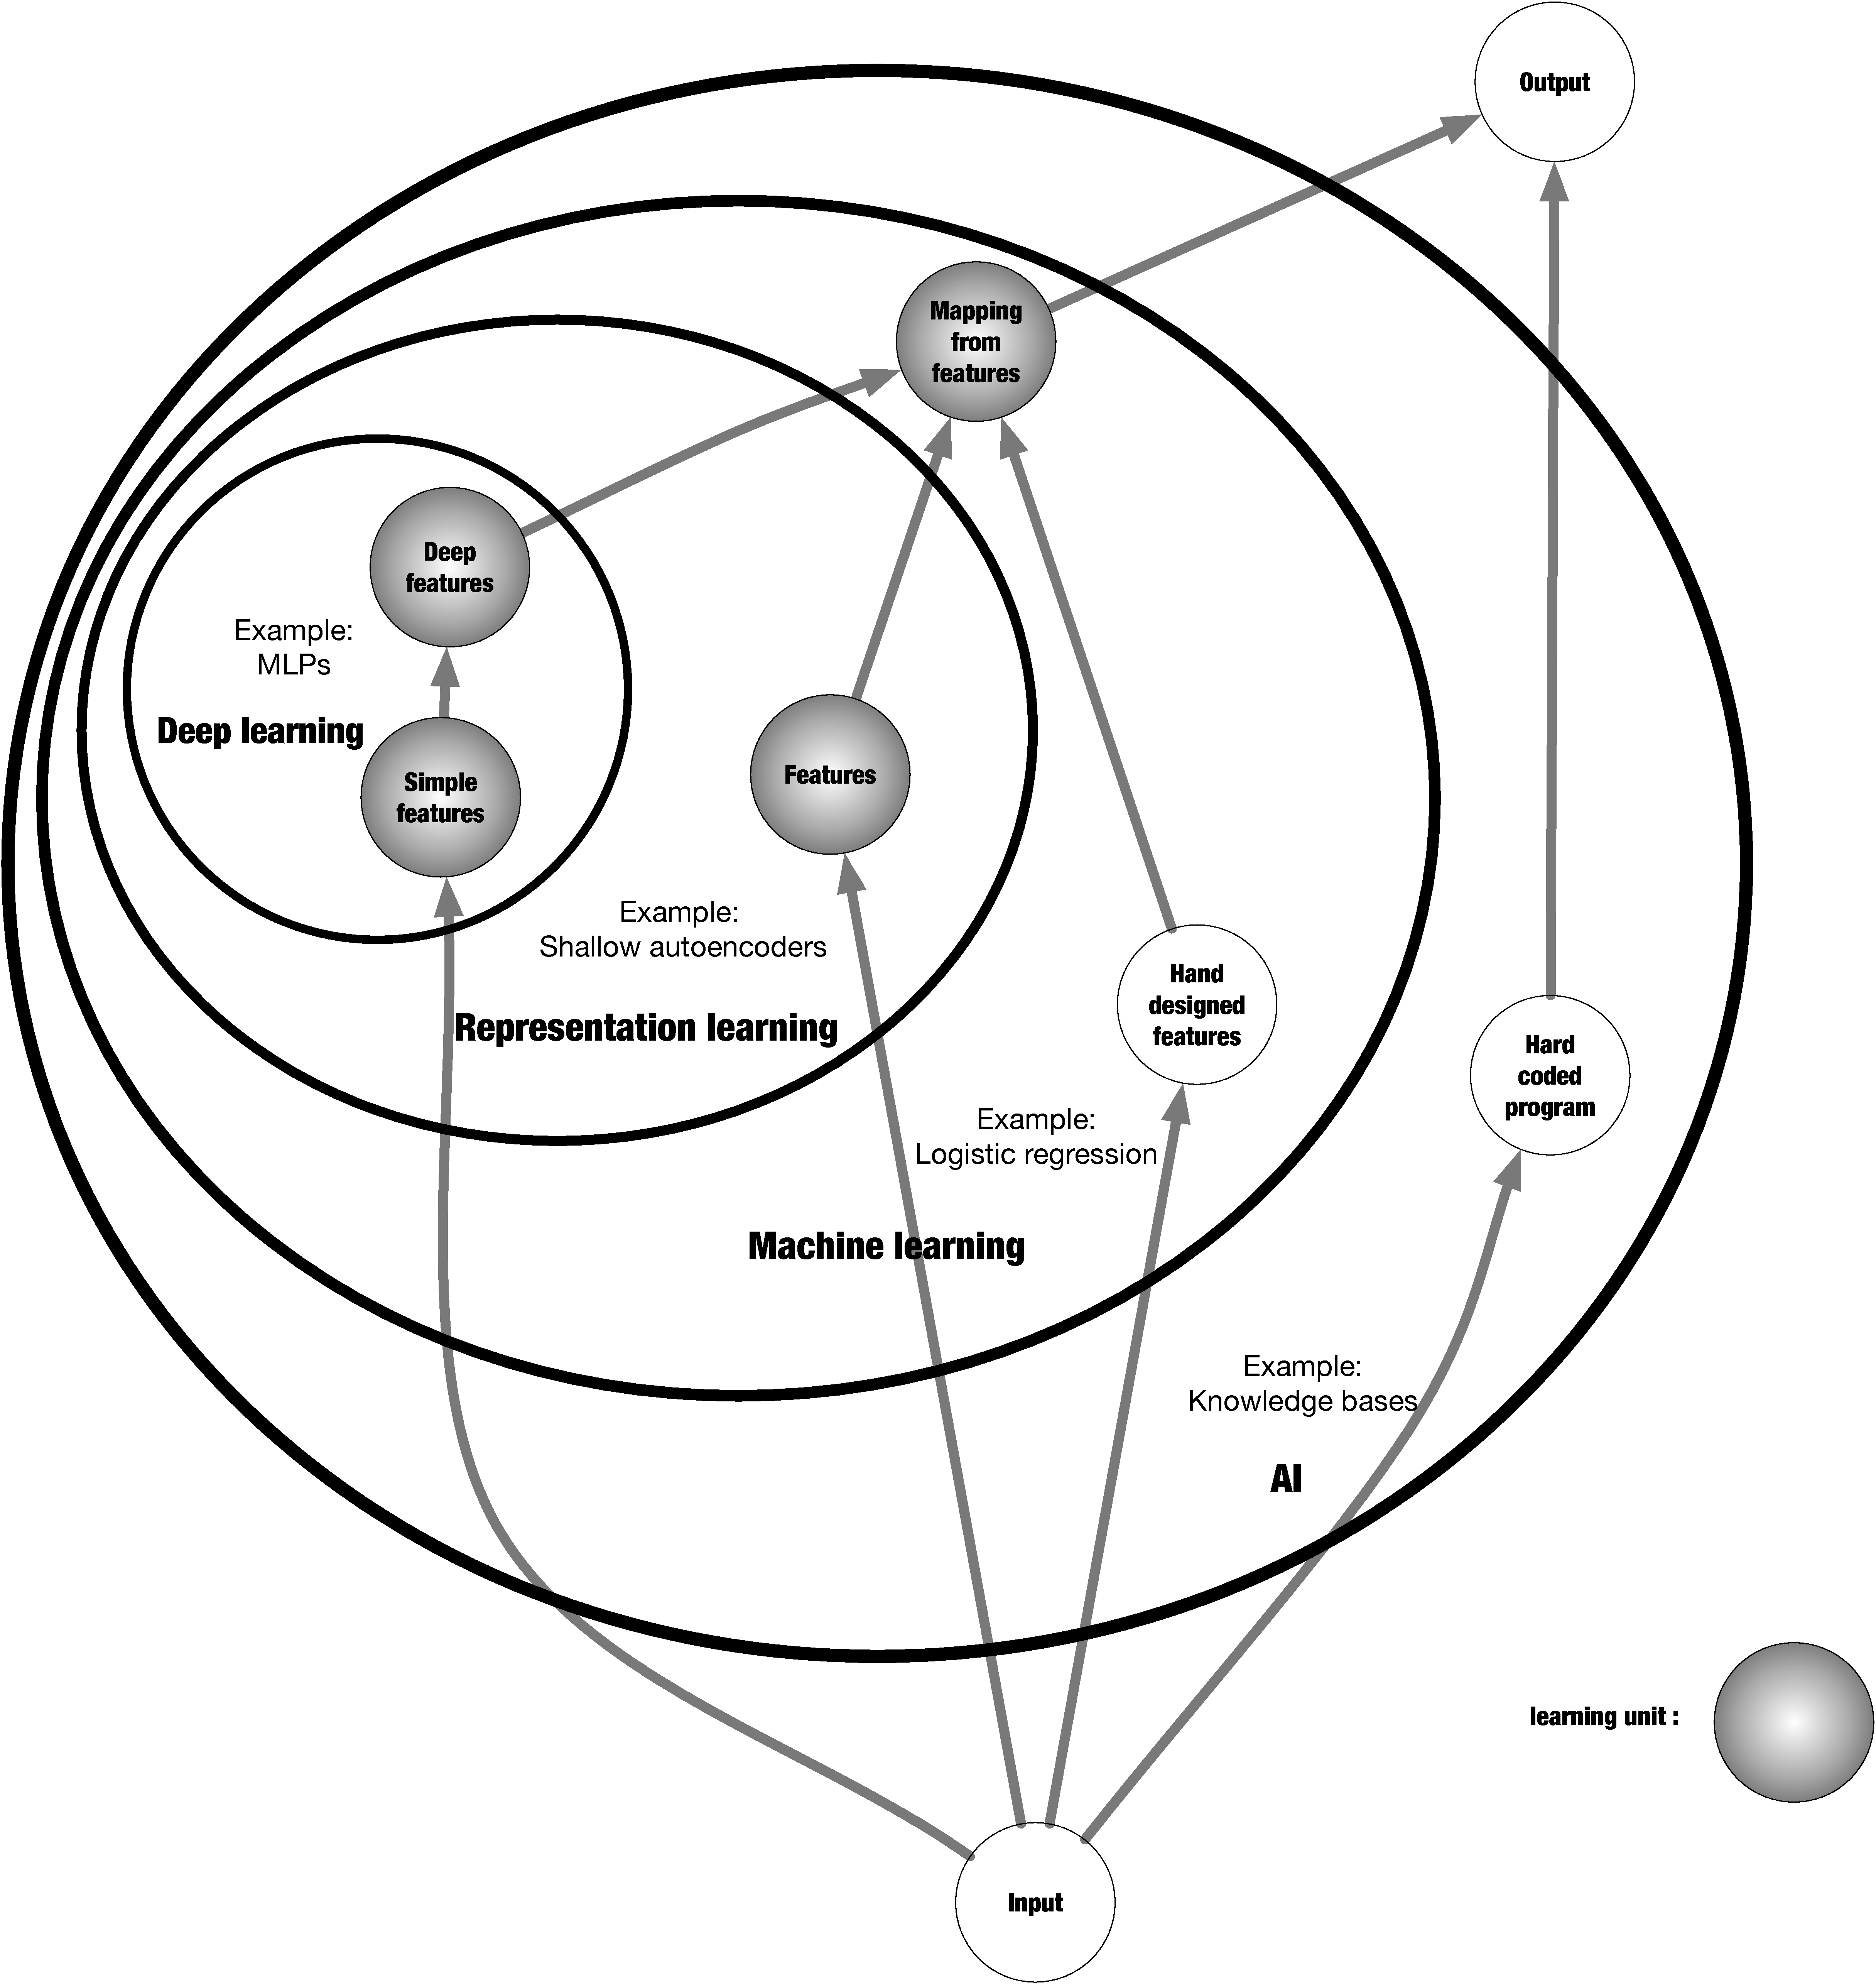
\includegraphics[width=0.5\textwidth]{figure/ch3-dlrelation.pdf}
    \caption{Venn diagram showing relations between deep learning, representation learning, machine learning, and AI. An example and work flow are also included for each section.}
    \label{fig:ch3-dlrelation}
\end{figure}

\subsection{Three Waves}
Deep learning has been rebranded many times under different names, only recently become well known as "deep learning". Broadly speaking, there have been three waves of development of deep learning: in 1940s-1960s known as \emph{cybernetics}~\cite{hebb2005organization, rosenblatt1958perceptron}, in 1980s-1990s known as \emph{connectionism}~\cite{rumelhart1985learning}, and the current resurgence starts from 2006~\cite{Hinton:2006:FLA,hinton2006reducing,Bengio07greedylayer-wise}. These three waves witness the evolving from simple perceptron, to distributed representation and stochastic gradient descent algorithm, and finally to today's various deep structures. The resurgence of deep learning benefits from the facts: computers are faster, datasets are bigger and a good initialization of model parameters. Faster computers make it possible to train deeper models, bigger datasets relieve deep models from overfitting, and enable them to learn more meaningful mid-level features that are more generalizable, and a good initialization through layer wise pretraining provides a proper prior and makes supervised training on later stages much easier.

Since the early stage of deep learning, neuroscience is regarded as an important source of inspiration. However, it is no longer a predominant guide for the field because we simply do not have enough information about the brain to use it as a guide. It is seemed as a more general principle of learning multiple levels of composition, which can be applied in machine learning frameworks that are not necessarily neurally inspired.


\subsection{Breakthroughs}
We highlight some of the breakthroughs brought by deep learning in recent years:
\begin{itemize}
\item In the ImageNet Large-Scale Visual Recognition Challenge (ILSVRC) 2012, a convolutional neuron network won this challenge for the first time and by a wide margin, bringing down the state-of-the-art top-5 error rate from 26.1\% to 15.3\%~\cite{krizhevsky2012imagenet}, since then the top-5 error rate keeps dropping down each year~\cite{SimonyanZ14a, szegedy2015going} and in last year dropped to 3.6\% using deep residual network (ResNet)~\cite{kmhresnet15}. Deep networks also had spectacular successes for pedestrian detection and image segmentation~\cite{sermanet2013pedestrian,farabet2013learning,couprie2013indoor} and yield superhuman performance in traffic sign classification~\cite{cirecsan2012multi}.
\item In March, Google DeepMind's AlphaGo defeated world champion Lee Sedol using deep reinforcement learning~\cite{silver2016mastering,links:alphagovslee}. Prior to that, they also showed that a deep reinforcement system is capable of learning to play Atari video games and reaching human-level performance on many tasks~\cite{mnih2013playing}.
\item The application of deep learning on other fields such as speech recognition~\cite{dahl2010phone, deng2010binary, hinton2012deep} and machine translation~\cite{sutskever2014sequence, bahdanau2014neural} all lead to great successes. The past years surfaced many new trends such as generative adversarial networks, neural Turing machines etc~\cite{goodfellow2014generative, radford2015unsupervised, graves2014neural, xu2015show, links:olah2016attention}. The years ahead are full of challenges and opportunities to improve deep learning even further and bring it to new frontiers.
\end{itemize}



\subsection{Artificial Neural Networks}

\subsubsection{A Single Neuron}
\begin{figure}[t]
    \centering
    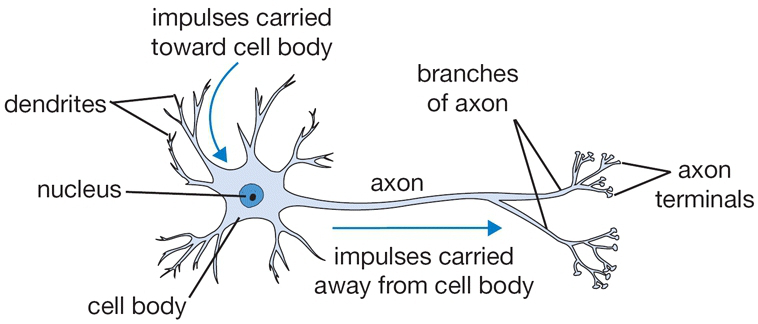
\includegraphics[width=0.45\textwidth]{figure/ch3-bioneuron.png}
    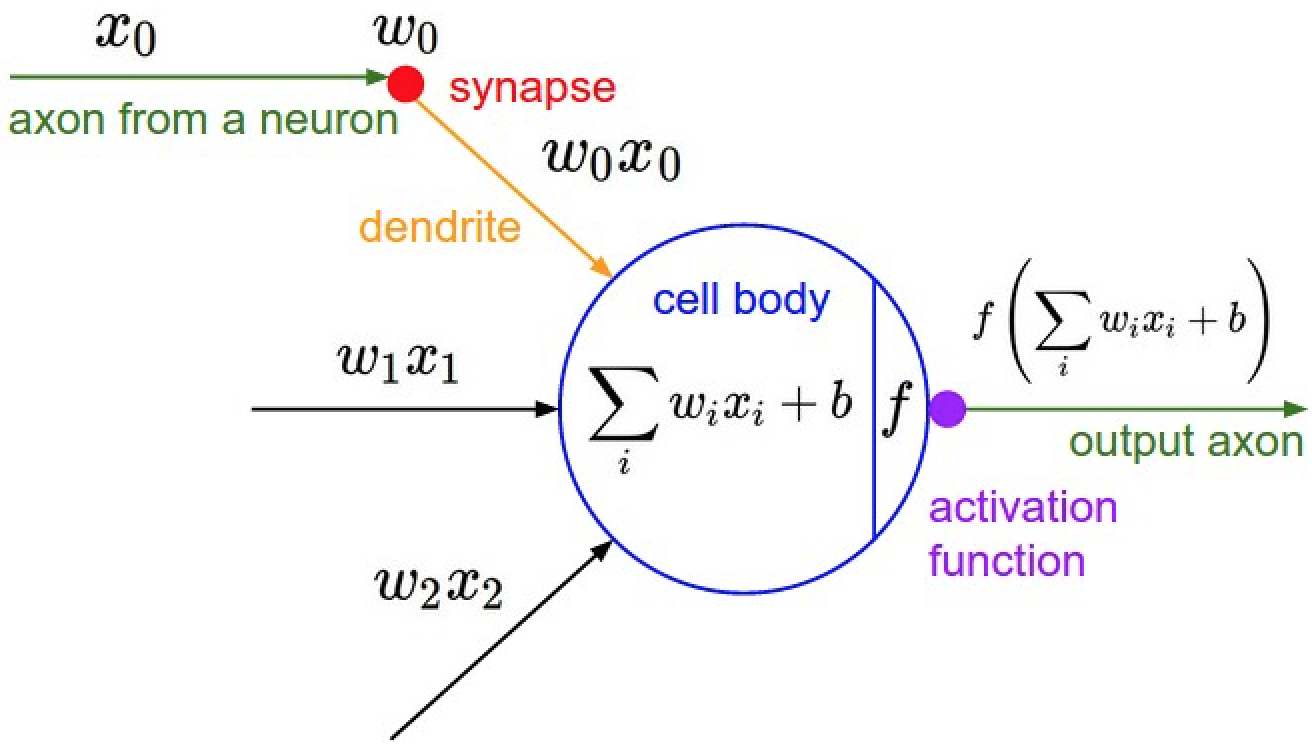
\includegraphics[width=0.45\textwidth]{figure/ch3-compneuron.png}
    \caption{A  cartoon drawing of a biological neuron (left) and its mathematical model (right). Photo taken from \emph{Module1: Neural Networks} in~\cite{links:cs231n}}
    \label{fig:ch3-neuron}
\end{figure}


Fig~\ref{fig:ch3-neuron} shows how to coarsely model a biological neuron: Each neuron receives input signals from its dendrites and produces output signals along its (single) axon. The axon eventually branches out and connects via synapses to dendrites of other neurons. In the basic model, the dendrites carry the signal to the cell body where they all get summed. If the final sum is above a certain threshold, the neuron can fire, sending a spike along its axon. In the computational model, we assume that the precise timings of the spikes do not matter, and that only the frequency of the firing communicates information. Based on this rate code interpretation, we model the firing rate of the neuron with an activation function $f$, which represents the frequency of the spikes along the axon. Historically, a common choice of activation function is the sigmoid function $\sigma$, since it takes a real-valued input (the signal strength after the sum) and squashes it to range between 0 and 1. Hereafter in this thesis, we will take standard naming convention and refer a hidden unit as a computational neuron.

\subsubsection{Activations}

\begin{figure}[!htbp]
    \centering
    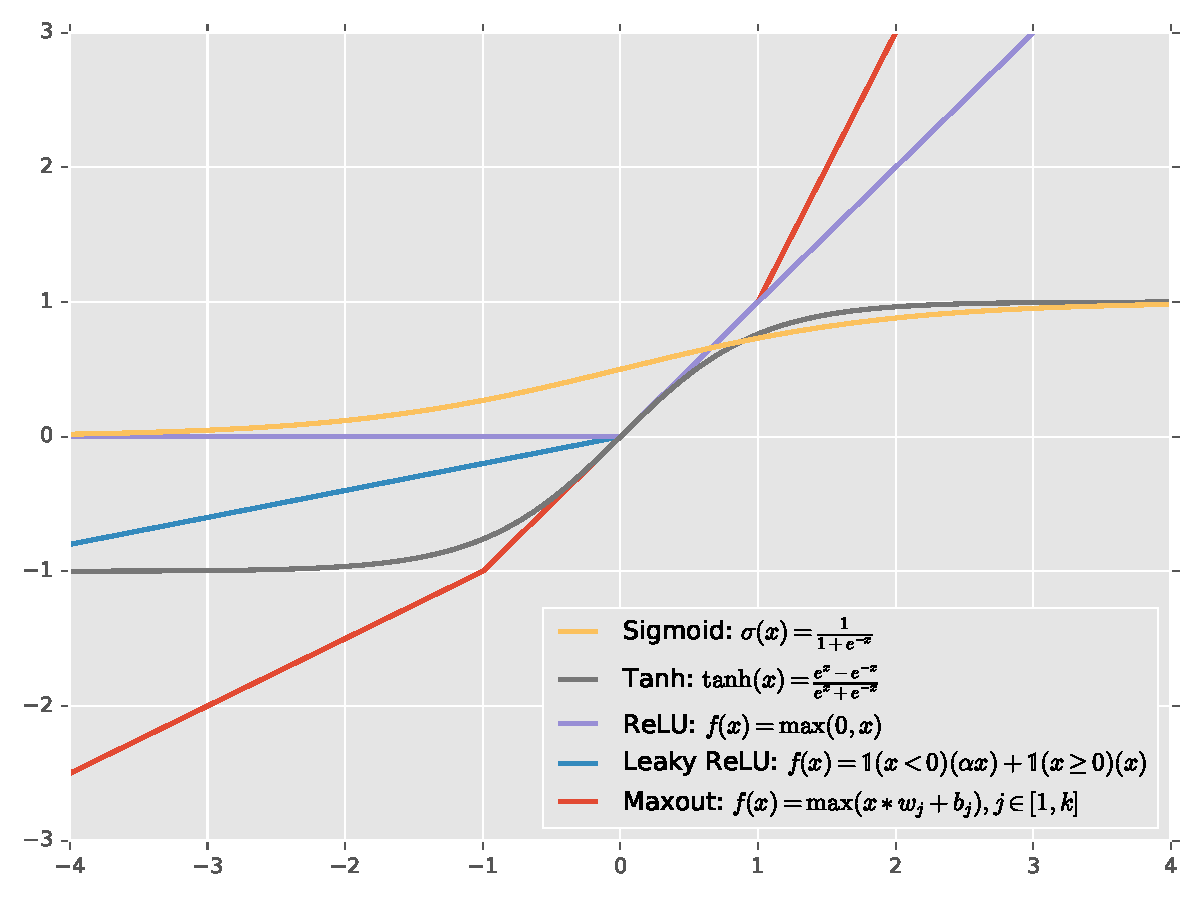
\includegraphics[width=0.6\textwidth]{figure/ch3-activations.pdf}
    \caption{Commonly used activation functions.}
    \label{fig:ch3-activations}
\end{figure}


Depends on the activation, neurons can have different properties and impacts on the whole network. Figure~\ref{fig:ch3-activations} shows most commonly used activation functions:

\begin{description}[labelindent=1cm]
  \item[Sigmoid] Sigmoid is used historically to simulate the firing rate of a neuron but recent years falls out of favor and is rarely used now. It saturates at either tail of 0 or 1, and at these regions the gradient is almost zero, thus it kills gradients from propagating to previous layers, making deep networks not trainable. Another drawback of sigmoid activation is that neurons in later layers will not receive zero-centered inputs, this will cause all positive or negative gradients on the weights during backpropagation, which may lead to undesirable zig-zagging dynamics in the gradient updates of the weights. However, once gradients are added up across a batch of data, the final update for the weights can have variable signs, somewhat mitigating this issue.
  \item[Tanh] Though similar to sigmoid non-linerality in that it also suffers from saturization and thus vanishing gradients problems, tanh is always preferred to sigmoid because its output is zero centered.
  \item[ReLU] Rectified linear unit becomes popular in recent years. \cite{krizhevsky2012imagenet} used it in their winning 2012 ImageNet competetion and found that it greatly accelerated the convergence of stochastic gradient descent optimization process. Also comparing to other activations, it is a much more light weight operation since it is a simple thresholding operation. However, ReLU unit can "die" if a large enough gradient changes the weights such that the neuron never activates on new data.
  \item[Leaky ReLU] Similar to ReLU, but can help fix the "dying ReLU" problem by modifying the flat side of ReLU to have a small gradient~\cite{he2015delving}.
  \item[Maxout] Introduced in~\cite{goodfellow2013maxout}, Maxout unit enjoys all the benefits of a ReLU unit, and does not have its drawbacks. Maxout activation can implement ReLU activtions and approximate any convex activation function.
\end{description}


\subsubsection{Basic Network Structure}
With appropriate loss function, a single hidden unit can function as a linear classifier. However, due to simplicity, its representation power is limited. For example, XOR operation can not be implemented with a single unit, but can be implemented with 3 units. For the network to have enough learning capacity to solve complicate tasks, hidden units are usually aggregated and stacked to form a layer by layer structure. With appropriate regularization, the network can learn powerful features and perform well for many tasks. A regular neural network is shown in Fig~\ref{fig:ch3-ann}, a deep neural network can have many hidden layers. \cite{links:nnplayground} provides an interactive play ground for tinkering with neural networks.


\begin{figure}[t]
    \centering
    \begin{tikzpicture}
        [nodestyle/.style = {circle, inner sep=0pt, minimum size=10pt},
         outstyle/.style = {-latex'new, arrowhead=0.2cm}]

        \foreach \name / \y in {1,...,10}
            \node[nodestyle, fill=black!50] (I-\name) at (0, -\y/2) {};

        \foreach \name / \y in {1,...,12}
            \node[nodestyle, fill=blue!50] (H-\name) at (2, -\y/2 + 0.5) {};

        \foreach \name / \y [count=\i from 0] in {1,...,10}
            \node[nodestyle, fill=red!50] (S-\name) at (4, -\y/2) {\i};

        \draw[dotted, thick, black!50] (I-10) ++(0cm,-0.3cm) -- ++(0cm, -1cm);
        \draw[dotted, thick, blue!50] (H-12) ++(0cm,-0.3cm) -- ++(0cm, -1cm);
        \draw[dotted, thick] (I-10) ++(0cm,-0.3cm) -- ++(0cm, -1cm);

        \foreach \source in {1,...,10}{
            \foreach \dest in {1,...,12}{
                \path (I-\source) edge[outstyle] (H-\dest);
                \path (H-\dest) edge[outstyle] (S-\source);
            }
        \draw[outstyle] (S-\source) -- ++(0.5cm, 0cm);
        }

        \node[text width=8em, text centered, above of=H-1, node distance=0.5cm, font=\tiny] (hl) {Hidden layer};
        \node[text width=8em, text centered, left of=hl, font=\tiny, xshift=-1cm] {Input image};
        \node[text width=8em, text centered, right of=hl, font=\tiny, xshift=1cm] {Output probabilities};

        \node[draw=blue!50, inner sep=0] (mnistres) [below right of=H-12, shift={(4cm,1cm)}] {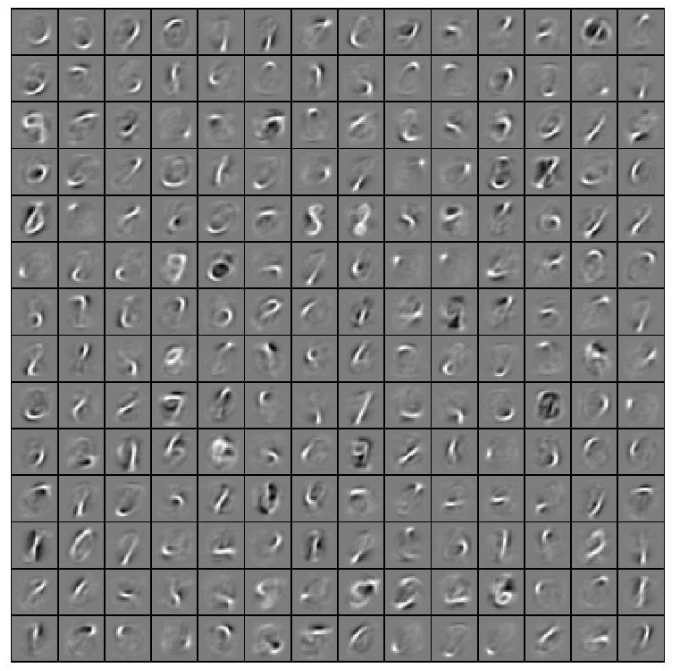
\includegraphics[width=3cm]{figure/dep/mnistresult.png}};
        \node[draw=black!50, inner sep=0] (mnistimg) [left of=I-4, shift={(-0.2cm,0)}] {
\includegraphics[width=1cm]{figure/dep/mnist.png}};
        \node[draw=blue!50, rectangle, inner sep=0, minimum width=0.5cm, minimum height=7.2cm] (fmaps) [above of=H-10, yshift=0.15cm] {};
        % \path (fmaps.north east)  edge [outstyle, bend left, blue!50, out=40] (mnistres.north);
        \node[draw=black!50, rectangle, inner sep=0, minimum width=0.5cm, minimum height=6.1cm] (aimg) [above of=I-9, yshift=0.15cm] {};
        \path (aimg.north west)  edge [outstyle, bend right, black!50] (mnistimg.north);
        \def\rectanglepath{-- +(0.2cm,0cm) -- +(0.2cm,0.2cm) -- +(0cm,0.2cm) -- cycle}
        \draw[blue!50, thick] (5.26, -5.41) \rectanglepath;
        \draw[rotate=45, blue!50, thick] (H-12) ++(-0.05cm, 0.3cm) ellipse (0.3cm and 0.1cm);
        \draw[outstyle, blue!50, decorate,
        decoration={snake,amplitude=.4mm,segment length=2mm,post length=1mm}]
        (H-12) ++(-0.5cm, -0.07cm) to [bend right] 
        node [below, text width=3cm, align=center, midway, font=\tiny]{kernel(feature filter)} (5.26,-5.31) ;

    \end{tikzpicture}

    \caption{A regular feed forward neural network with 1 hidden layer. A 28x28 mnist digit image is flattened and fed into the network, it outputs probabilities of being a certain digit from 0 to 9. The learned kernel for each hidden unit is also shown.}
    \label{fig:ch3-ann}
\end{figure}

\subsubsection{Backpropagation Algorithm}
During the optimization process of loss function, we need to calculate the gradients with respect to all the weights and update them. A naive way is keep all the weights fixed and only tweak one weight to see how it changes loss, thus get its gradient. However, this method is very inefficient since it has to tweak order of the number of weights times to get gradients for all the weights. The efficient way to do this is backpropagation algorithm. Detailed derivations on backpropagation algorithm can be found on tutorials~\cite{links:nielsennnbook, links:cs231n}. We highlight some points here:
\begin{itemize}
\item It helps to think of the mapping from input to output that the neural network represents as a computational graph. Each node in this computational graph is simple operation like $+$, $*$, $\max$, or any operation like $\sigma$ that have a simple derivable gradients. In such way, any complicate mapping function is decomposed into simple unit operations, and backpropagation refers to the node by node backward propagation of gradients from loss to input using chain rule.
\item There can be many paths from loss to any variable in the network, gradients flowed through all these paths backwards to this variable get added up when calculating gradient on this variable.
\item In neural networks, the preactivations of a layer $z$ and activations of previous layer $o$ have relation $z = w^To$ where $w$ are the weights between these two layers, it can be seen that gradients for $w$ are proportional to activations $o$ of previous layer, this implies that the scale of the data has an effect on the magnitude of gradients for the weights. When input data is not scaled well, the gradient can be huge, so data preprocessing is a good practice.
\end{itemize}

\subsubsection{Training}
Below we list most of the practical concerns when training neural networks:
\begin{description}[labelindent=1cm]
  \item[Data Preprocessing] Common data preprocessing steps include mean subtraction, normalization, PCA whitening~\cite{links:ufldlpca}. Mean subtraction is to zero-center the data. Normalization refers to normalizing the data dimensions so that they are of approximately the same scale. PCA whitening is to first apply PCA on the dataset, followed by a normalization step on the principle components. For most computer vision tasks with big image datasets as input, mean subtraction is enough.
  \item[Weight Initialization] Mostly used weight initialization strategy is random sampling from a damped gaussian distribution. Improvements on randomly initialization are focused on calibrating the variances with respect to number of inputs for each neuron such that its output's variable does not blow up. For ReLU units, it is recommended to draw weights from $\sqrt{\frac{2.0}{n}}\mathcal{N}(0,1)$ as suggested in~\cite{he2015delving}. A recently developed technique called batch normalization explicitly forces each neuron's activations for a minibatch to take on a unit gaussian distribution through whitening among this minibatch~\cite{ioffe2015batch}. Batch normalization can be interpreted as doing preprocessing at every layer of the network, but integrated into the network itself in a differentiable manner. In practice networks that use batch normalization are significantly more robust to bad initialization.
  \item[Regularization] $\mathcal{L}2$ regularization $\frac{1}{2}\lambda w^2$ is still the most commonly used regularization term. Other than that, $\mathcal{L}1$ regularization $\lambda |w|$ leads to sparsity in weights, it is useful when the problem is concerned with explicit feature selection. Dropout~\cite{srivastava2014dropout} is a simple but effective way of regularization, in practice it smears activations with a certain probability during training, which can be interpreted as sampling a neural network within the full neural network, and only updating the parameters of the sampled network based on the input data, therefore effectively there are many more neural nets working as an ensemble to eventually perform the classification.
  \item[Loss Functions] In classification problems, most commonly used data loss functions are hinge loss and cross-entropy loss. Hinge loss is defined as $L_i = \sum_ {j\neq y_i} \max(0, f_j-f_{y_i}+1)$ where $L_i$ and $y_i$ refer to loss and ground truth label of $i$th sample, $f_j$ is the output score for class $j$. Hinge loss is used with SVM classifier. Cross-entropy loss is defined as $L_i = -\log(\frac{e^{f_{y_i}}}{\sum_je^{f_j}})$, and used with Softmax classifier. For regression problems, $\mathcal{L}2$ distance $L_i = ||f - y_i||_2^2$ are normally used. Whenever possible, it is recommended to see if a regression problem can be morphed to a classification problem by quantization of outputs into bins, because classification is an easier task and gives confidences of each class.
  \item[Optimization] There are many optimization options when training deep neural networks. Starting from vanilla SGD (stochastic gradient descent), integration of momentum improves convergence rate and adaptive algorithms ease the pain of tuning the learning rates. \cite{links:sgdoptimization}~gives a comprehensive overview of related algorithms.
  \item[Miscellous] To find good hyperparameters such as initial learning rate, regularization strength, it is suggested to use random search over grid search~\cite{bergstra2012random} and stage the search from coarse to fine. Bagging of neural networks trained independently is a reliable approach to improve the performance.
\end{description}


\section{Convolutional Neural Networks}

\subsection{Architecture Overview}

\subsection{Layers}

\section{Applications}

\subsection{Classification}

\subsection{Detection}


\newpage
